\documentclass{article}

\usepackage{pgf}
\usepackage{tikz}
\usetikzlibrary{arrows,automata}
\usepackage[latin1]{inputenc}
\begin{document}
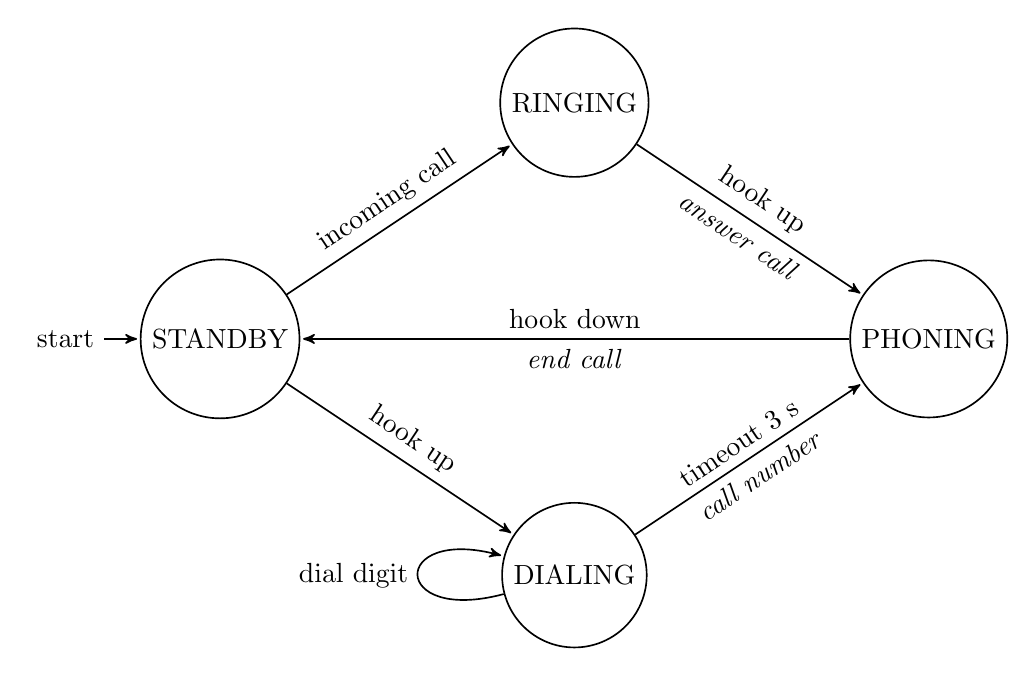
\begin{tikzpicture}[->,>=stealth',shorten >=1pt,auto,node distance=2.8cm,
                    semithick]
  %\tikzstyle{every state}=[fill=red,draw=none,text=white]

  \node[initial,state] (SB) at (0,3) {STANDBY};
  \node[state]         (RI) at (4.5,6) {RINGING};
  \node[state]         (DI) at (4.5,0) {DIALING};
  \node[state]         (PH) at (9,3) {PHONING};

  \path (SB) edge node [sloped]{incoming call} (RI)
             edge node [sloped] {hook up} (DI)
        (RI) edge node [sloped,above]{hook up} node [sloped, below]{\textit{answer call}} (PH)
        (PH) edge node [above]{hook down} node [below] {\textit{end call}} (SB)
        (DI) edge node [sloped, above] {timeout 3 s} node [sloped, below] {\textit{call number}} (PH)
	     edge [loop left] node {dial digit} (DI);
\end{tikzpicture}

\end{document}
